\chapter{Introduction}
%%\minitoc
{\scshape The inability to explain} the \emph{apparent} with the
knowledge of the \emph{real} is defined as Magic. And it is no
less magical to find the \emph{apparent} breaking of the orthodox
biological rules by which life survives under \emph{apparently
unusual} circumstances. The english word \emph{extreme} came from
roman \emph{extremus}, the superlative of \emph{exter}, meaning
\emph{being on the outside}. \emph{Extremophiles}, a term coined
by \citet{MacElroy1974}, are the lovers (\emph{philos} to the
Greeks) of \emph{extreme} environments. These \emph{outsiders}
extend the limits of biology in spite of being governed by strict
physical rules. Bound by unbreakable barriers, \emph{reaching out}
requires ingenuity. And when survival is at stake, given enough
time and trials, chance alone can be highly ingenious to turn
going astray into highly directional movement through rules laid
down by physics, as shown by Evolution.

Evolution is winning at any cost, if not by breaking the
fundamental rules of the physical universe, by bending them. A
complete overhauling of the biological machinery is called upon
when it comes to deal with the physical constraints created by
physics on perhaps the single most important substance for life,
the water.

Terrestrial Life evolved as the chemistry of water. Water in
liquid form is the most important substance for sustenance of life
on Earth. Although, solid ice is widespread in Solar System,
liquid water is evanescent; can persist only in atmospheric
pressure \U{>6}{mbar}. Liquid water is available only on the
surface of Earth, because, the size of Earth and distance of Earth
from Sun are just perfect to keep water in liquid
form~\citep{Brack1998}. And life flourishes wherever water exists
in liquid form.

Temperature, as a physical factor, has the greatest influence on
the properties of the water. From vapor-liquid-solid phase
transitions to pH, from density to solubility, almost every aspect
of water chemistry is changed with the change of temperature.
Temperature also changes the most important property of water, the
H-bonding. Extremes of temperatures have potential devastating
effect on life forms. Structural devastation through the formation
of ice crystals on one extreme, to denaturation of biomolecules at
the other. Yet in nature we find organisms with thermal
preferences for all ranges. \emph{Pyrolobus fumarii}, a nitrate
reducing chemolithotroph archeon belonging to Crenarchaeota, grows
at 113\dg{}, the upper temperature limit of life till
date~\citep{Blochl1997}. \emph{Panagrolaimus davidi}, an Antarctic
nematode withstand freezing of all body water~\citep{Wharton1995}.
Active microbial community has been found at
$-$18\dg{}~\citep{Rothschild2001}.

To thrive under these conditions, each organism has to carry out
the routine biological activities, which largely depend on
specific advantageous modifications to the biological machinery.
These modifications, loosely termed as \e{adaptations}, are
intriguing, from the view point of sheer complexity and ingenuity.

Transcription is one of the functions that these organism has to
carry out, no matter what the environment be. Carrying out by RNA
polymerase, cellular RNA synthesis is also a step which is highly
controlled by environmental cues. A particular subunit of this
highly complex enzyme is \s{} factor, which play a cardinal role
in functioning of this enzyme. The work presented in this thesis
examines the role of a particular \s{} factor, \sigs{}, which is
known to be the central character in variety of stress conditions,
in the adaptation of a cold-adapted extremophile, \e{Pseudomonas
syringae} strain Lz4W from Antarctica. The present work also looks
into the features of the major or the vegetative \s{} subunit,
\s\su{D}, which regulates the expression of \e{house-keeping}
genes in bacterial cell, from this extremophile.

In this Chapter, after a brief introduction to cold-adaptation in
bacteria, the summary of a very recent breakthrough on the
structure of RNA polymerase is discussed, in the context of its
function. After this summary, a detailed discussion on \s{} factor
structure and function, followed by a discussion on its
classification, the present knowledge about the \sigs{} regulation
is presented. Lastly, the objectives of the present study are
stated.


\section{Thermal preference of bacteria}

Depending on the ability to grow at various temperatures
microorganisms have been divided into five categories
(Table~\ref{chap1_therm}). Among them, cold-adapted bacteria
belong to two categories: \e{psychrophiles} and
\e{psychrotrophs}~\citep{Morita1975}. Both these categories
consist of extremely diverse genera, which probably employ common
molecular mechanisms that allow maintenance of vital cellular
functions at low temperature. Psychrotrophic bacteria are more
ubiquitous than psychrophiles. They also have widest of growth
ranges (up to 40\dg{}) of all the known bacterial
species~\citep{Hebraud1999}.

\begin{table}[tbp]
\linespread{1}\normalsize
\renewcommand{\arraystretch}{1.2}
\begin{minipage}[c]{\textwidth}
\renewcommand{\footnoterule}{}
\renewcommand{\footnotesep}{0pt}
\caption[Bacterial classification based on growth temperature]
{Bacterial classification based on growth temperature}
\label{chap1_therm}
\begin{narrow}{-1in}{-1in}
\centering
\begin{small}
\begin{tabularx}{\textwidth}{@{}cccc@{}}\toprule
\textbf{Category} & \textbf{Minimum (\dg{})} & \textbf{Optimum
(\dg{})} & \textbf{Maximum (\dg{})} \\\midrule
Hyperthermophile & $\sim$55 & 80--110 & 113 \\
Thermophile & $\sim$45 & 50--70 & $\sim$80 \\
Mesophile & $\sim$10 & 30--40 & $\sim$45 \\
Psychrotroph & $\leq$0 & 20--25 & $\sim$35 \\
Psychrophile & $\leq$0 & $\leq$15 & $\sim$20 \\\bottomrule

\end{tabularx}
\end{small}
\end{narrow}
\end{minipage}
\renewcommand{\arraystretch}{1.0}
\linespread{1.1}\normalsize
\end{table}


\section{Antarctic psychrotoph \emph{Pseudomonas syringae} Lz4W}
Bacteria from Antarctica represent both psychrophiles and
psychrotrophs~\citep{Wynn1990}. The present work was carried out
on a psychrotrophic bacterium originally classified as
\e{Pseudomonas syringae} Lz4W, which is being used as a model
system for understanding the molecular basis of cold-adaptation,
in our laboratory~\citep{Ray1998}. For all further discussion,
this organism will be referred to as Lz4W. This organism was
isolated from soil samples collected from Schirmacher Oasis region
of Antarctica~\citep{Shivaji1989}. This region is unique in that
it is as cold as the rest of the continent, but is under ice-cover
only during Antarctic winter, and experiences significant
precipitation~\citep{Shivaji1989}. Lz4W has optimal growth
temperature range of 20--25\dg{} and a maximal growth temperature
of about 30\dg{}. Lz4W grows with a generation time of $\sim$100
minutes at 22\dg{} and $\sim$250 minutes at 4\dg{} in rich medium.

\section{Strategies of cold-adaptation}

In order to put the objectives of the present study in proper
perspective, it is necessary to give an account of the present
knowledge of cold-adaptation. There are several mechanisms by
which bacteria adapt to low temperature. In this Section a very
brief summary is presented.

\subsection{Membrane fluidity at low temperature}

One of the best studied mechanisms by which bacteria adapt to low
temperature is maintenance  of an optimal degree of fluidity in
membranes~\citep[reviewed in][]{Russell1990a,Russell1998}. There
are several ways this can be achieved, such as, by increasing
unsaturated fatty acid content, increasing \e{cis} double bonds,
chain-shortening, and in some cases methyl-branching. In this
aspect, the cold-induced \e{des} genes, which have been identified
to encode membrane phospholipid desaturases from a variety of
organisms, are known to play a very vital role in genetic
regulation of membrane fluidity~\citep[for a recent review
see][]{Sakamoto2002}.

\subsection{Cold-adapted enzyme}

Compared with their mesophilic counterparts, enzymes from
cold-adapted bacteria are more thermolabile but possess a very
high specific activity and catalytic efficiency at low
temperature~\citep[reviewed
in][]{Feller1997,Gerday1997,Lonhienne2000}. In general, two types
of adaptive mechanisms have been noticed. First, the enzymes have
evolved towards the lowest possible stability in the native state.
Second, the proteins have acquired higher flexibility resulting in
the appearance of a distinct thermodynamically heat-labile
domains. Flexibility is more apparent near the catalytic site
reducing the activation energy, thus increasing the reaction rate
(K\sub{cat}/K\sub{m}) at low temperature.

\subsection{Cold-shock response}

When growing culture of bacteria is suddenly shifted to
temperature below the cardinal growth, they exhibit cold-shock
response~\citep{Jones1987}. The response is characterized by a
transient growth-arrest during which a number of genes are
induced, in contrast to a severe inhibition of general protein
synthesis. In \bact{Ec}, the major cold-shock protein (CSP) is
CspA, which constitutes almost 10\% of cellular protein content
during cold-shock~\citep{Goldstein1990}. Other cold-inducible
proteins include, transcription factor NusA, polynucleotide
phosphorylase, initiation factor IF2, RecA, H-NS, DNA gyrase,
ribosome associated factor RbfA and RNA helicase
CsdA~\citep[reviewed in][]{Yamanaka1999}.

In \bact{Ec}, there are nine Csp proteins, from CspA through CspI,
of which CspA, B, G and I are cold-shock inducible. CspC and E are
constitutively produced at 37\dg{}, whereas CspD is induced upon
nutritional deprivation. The induction pattern of CspF and H are
not known~\citep[reviewed in][]{Phadtare1999a}. CspA homologs are
widely distributed in prokaryotes and homologous to Y-box proteins
in eukaryotes. None of the CspA homologs are singularly
responsible for cold-shock adaptation, because deletions in any
one the \e{csp} genes does not result in cold
sensitivity~\citep{Xia2001}. The double deletion mutants
($\Delta$\emph{cspA}$\Delta$\emph{cspB},
$\Delta$\emph{cspA}$\Delta$\emph{cspG},
$\Delta$\emph{cspA}$\Delta$\emph{cspI},
$\Delta$\emph{cspB}$\Delta$\emph{cspG}) and triple deletion
mutants
($\Delta$\emph{cspA}$\Delta$\emph{cspB}$\Delta$\emph{cspG}) of
\bact{Ec} are not cold sensitive, whereas the quadruple deletion
mutant is cold sensitive. In \bact{Ec} deleted for \emph{cspA},
\emph{cspB} and \emph{cspG}, CspE accumulates at low temperatures
suggesting that the members of the cold-shock family may
functionally substitute each other during cold acclimation of
cells~\citep{Xia2001}.

Csp family members have been shown to bind RNA and single stranded
DNA \citep{Phadtare1999}. CspE in \bact{Ec} has been shown to be
involved in transcription elongation by acting as an
antiterminator~\citep{Phadtare2002}. The physiological function of
Csp family in cold-adaptation, however, is largely unknown.

Psychrotrophic bacteria also exhibit a cold-shock response, when
suddenly exposed to low temperatures (such as, a shift from 22 to
4\dg{}). Genes homologous to CspA are found in several cold
tolerant bacteria including \e{Pseudomonas} \citep{Ray1994},
\e{Arthrobacter}, \e{Listeria}, \e{Bacillus cereus},
\e{Micrococcus roseus}~\citep{Hebraud1999}. But an important
feature of the cold-shock response in cold-adapted bacteria is
that house-keeping genes are not repressed during the response,
suggesting translation apparatus is suitably adapted to fuction at
low temperature in this bacteria. Many of the Csp homologs are
also continuously synthesized during growth at low
temperature~\citep{Hebraud1999}.

\subsection{Cold-acclimation proteins}

At low temperature, the psychrotrophs and psychrophiles also
produce a specific set of proteins that are absent or poorly
present at higher temperature, known as cold acclimation proteins
(CAPs). These classes of proteins are  constitutively synthesized
throughout the growth at low temperature. The CAPs are thought to
play an important role in the cellular physiology in cold. The
synthesis of CAPs are graded, with different subset of proteins
made to different extent during growth at low
temperature.~\citep{Hebraud1999}.

\section{A cold-active RNA polymerase}

As regulation of gene expression plays a major role in
cold-adaptation, it is important to understand the nature of the
transcription machinery from the cold-adapted bacteria. Very
little, however, is known about the the nature of the RNA
polymerase from these organisms. Purified RNA polymerase from Lz4W
exhibited a typical eubacterial subunit composition with
$\betaup$, $\betaup'$, $\alphaup$\sub{2} and \s{} subunits. The
$\alphaup$ subunit of Lz4W RNA polymerase was larger (\U{45}{kDa})
than $\alphaup$ of \bact{Ec} (\U{37}{kDa}). The subunits
cross-reacted with antibodies raised against \bact{Ec} RNA
polymerase~\citep{Uma1999}.

The RNA polymerase of Lz4W was, however, unique in its ability to
transcribe at 0\dg{}, albeit at lower efficiency (10--15\%)
compared with its activity at 37\dg{}\@. The enzyme was
thermolabile; it lost 50\% of its activity at 45\dg{} within 30
minutes. The most important feature of this RNA polymerase was
that it could preferentially transcribe cold-inducible \e{cspA}
gene of \bact{Ec} only at lower temperature. It also became
relatively more rifampicin resistant during transcription at low
temperature~\citep{Uma1999}.


\section{Multisubunit RNA polymerase}

Transcription is the first step in gene expression. RNA polymerase
(RNAP), the enzyme responsible for transcription, is targeted,
directly or indirectly during regulation of gene expression. RNAPs
is conserved in all organisms~\citep{Ebright2000,Young1991}. RNAPs
from three phylogenetic domains of life, Eubacteria, Archaea, and
Eukaryota, belong to a conserved protein family, termed the
\emph{multisubunit RNAP family}. In Eubacteria and Archaea, a
single multisubunit RNAP is responsible for synthesis of all
cellular RNA. In eukaryotes, three distinct multisubunit RNAPs are
found within the cell nucleus. RNAPI synthesizes rRNA, RNAPII
synthesizes mRNA, and RNAPIII synthesizes 5S RNA, tRNA, and some
small nuclear RNAs.

Members of the multisubunit RNAP family contain a conserved
subunit of \U{$\sim$160}{kDa} ($\betaup'$ in bacterial RNAP; A in
archaeal RNAP; RPAI, RPBI, and RPCI in eukaryotic RNAP I, II and
III), a conserved subunit of \U{$\sim$150}{kDa} ($\betaup$ in
bacterial RNAP; B in archaeal RNAP; RPA2, RPB2, and RPC2 in
eukaryotic RNAP I, II, and III), a conserved subunit of
\U{$\sim$35}{kDa} ($\alphaup$I in bacterial RNAP; D in archaeal
RNAP; RPC5 in eukaryotic RNAP I and III; RPB3 in eukaryotic RNAP
II), a conserved subunit of \U{$\sim$10--35}{kDa} ($\alphaup$II in
bacterial RNAP; L in archaeal RNAP; RPC9 in eukaryotic RNAP I and
III; RPB11 in eukaryotic RNAP II) and a conserved subunit of
\U{$\sim$6}{kDa} ($\omegaup$ in bacterial RNAP; K in archaeal
RNAP; RPB6 in eukaryotic RNAP I, II, and
III)~\citep[][Table~\ref{pol_subunit}]{Ebright2000,Young1991}.

\begin{table}[tbp]
\linespread{1}\normalsize
\renewcommand{\arraystretch}{1.5}
\begin{minipage}[c]{\textwidth}
\renewcommand{\footnoterule}{}
\renewcommand{\footnotesep}{0pt}
\caption[Subunits structure of RNA polymerase]{Subunit structure
of multisubunit RNA polymerase family from three domains of
life~\citep{Ebright2000,Young1991}. $\alphaup$I and $\alphaup$II
are same proteins in bacteria.} \label{pol_subunit}
\begin{narrow}{-1in}{-1in}
\centering
\begin{small}
\begin{tabularx}{5.75in}{@{}>{\raggedright\arraybackslash}p{1.5in}%
>{\raggedright\arraybackslash}X%
>{\raggedright\arraybackslash}X%
>{\raggedright\arraybackslash}X%
>{\raggedright\arraybackslash}X%
>{\raggedright\arraybackslash}X%
>{\raggedright\arraybackslash}p{1in}%
@{}}\toprule \textbf{RNA polymerase (RNAP)} &
\multicolumn{5}{c}{\textbf{Conserved subunits}} &
\textbf{Non-conserved}\\\midrule Bacterial RNAP & $\alphaup$I &
$\alphaup$II & $\betaup$ & $\betaup'$
& $\omegaup$ & $+\sigmaup$\\
Archaeal RNAP & D & L & B & A$'$/A$''$ & K & $+$6 others \\
Eukaryotic RNAPI & RPC5 & RPC9 & RPA2 & RPAI & RPB6 & $+$9 others
\\
Eukaryotic RNAPII & RPB3 & RPB11 & RPB2 & RPB1 & RPB6 & $+$7
others \\
Eukaryotic RNAPIII & RPC5 & RPC9 & RPC2 & RPC1 & RPB6 & $+$11
others \\\bottomrule
\end{tabularx}
\end{small}
\end{narrow}
\end{minipage}
\renewcommand{\arraystretch}{1.0}
\linespread{1.1}\normalsize
\end{table}

The bacterial RNAP contains a catalytic core of \U{$\sim$400}{kDa}
(E; subunit composition
$\alphaup$\sub{2}$\betaup\betaup'\omegaup$). The binding to
promoter requires the $\sigmaup$ subunit, which binds to core to
form the holoenzyme (E$\sigmaup$). Each of these proteins is
produced by separate genes. In Gram-negative bacteria, the gene
names start with prefix ``\emph{rpo}''. The subunits, $\alphaup$,
$\betaup$, $\betaup'$, and $\omegaup$ are coded by \emph{rpoA},
\emph{rpoB}, \emph{rpoC}, and \emph{rpoZ}, respectively. The
nomenclature of $\sigmaup$ gene varies, with $\sigmaup$\su{70},
coded by \emph{rpoD}, being the major house-keeping $\sigmaup$
factor in \bact{Ec} and related bacteria.

\section{Transcription cycle}

The transcription cycle in bacterial cell has three main stages:
initiation, elongation and termination. Although, catalytically
active, the core enzyme is incapable of initiating transcription
efficiently and with specificity. For this, it requires initiation
factor, $\sigmaup$, to form holoenzyme (E\s{}) that can recognize
specific DNA sequences, called promoters~\citep{Burgess1969}.

During initiation, different $\sigmaup$ factors direct the
holoenzyme to bind to different types of DNA sequences (see
Table~\ref{sigma_promoters}). The $\sigmaup$\su{70} containing
holoenzyme binds to two conserved hexamers of DNA sequence: the
Pribnow box or the ``$-$10 element'', and the ``$-$35 element''
with respect to transcription start site ($+$1). The resulting
holoenzyme-DNA complex is called \emph{closed promoter
complex}~\citep{dehas1998}. A series of isomerization steps then
lead to the unwinding of double-stranded DNA between $-$12 to $+$2
of the promoter, resulting in \emph{open promoter complex}.
Transcription process starts in presence of nucleotide
triphosphate (NTPs) substrates. At this stage, the enzyme
repeatedly produce short, usually 2--12 nucleotides long
transcripts~\citep{Car1980} without dissociating from the promoter
(abortive transcription). By the time transcript reaches 12
nucleotides, the transcription process passes from the initiation
to the elongation stage~\citep{von1998}. This transition is
characterized by the escape of the RNA polymerase from the
promoter, the dissociation of \s{} from the core enzyme and
formation of a highly processive ternary elongation complex. There
is, however, a proposed alternative model, which proposes that
\s{} factor remains bound to the core enzyme in the elongation
complex~\citep{Bar2001}. At the termination stage, RNAP
dissociates from the DNA in response to specific termination
signal.

Evidently, the \s{} factor has a central role in the initiation
process, being directly involved in promoter recognition, DNA
melting and promoter escape and
clearance~\citep{Gross1998,Helmann1988}.

\section{RNA polymerase structure-function}
\label{crystal}

Since the initial indications of DNA-dependent RNAP activity from
a number of systems~\citep{Weiss1959,Huang1960,Hurwitz1960}, and
its first isolation from \bact{Ec}~\citep{Chamberlin1962}, a
wealth of biochemical, biophysical, and genetic information has
accumulated on RNAP and its accessory
factors~\citep{von1984,Erie1992,Gross1996a}. However, till very
recently, the enzyme itself, in terms of its structure-function
relationship, remained a black-box.

A first glimpse of a subunit of RNA polymerase came from the
determination of crystal structure of a fragment of \bact{Ec}
$\sigmaup$\su{70} subunit~\citep{Malhotra1996}. Soon after, that
the structure of \bact{Ec} RNAP core enzyme was determined at
\U{12}{\AA}~\citep{Darst1998}. However, a milestone in our
understanding of the multisubunit RNAP family was reached in 1999,
with the determination of a crystal structure of \emph{Thermus
aquaticus} RNAP core enzyme at \U{3.3}{\AA}
resolution~\citep[][PDB accession 1DDQ]{Zhang1999}. Subsequent
determination of crystal structures of yeast
RNAPII~\citep{Cramer2001} and the RNAPII in elongation
complex~\citep{Gnatt2001} from \emph{Saccharomyces cerevisiae}
revealed the high degree of similarity between the prokaryotic and
eukaryotic RNAPs.

Crystal structure of bacterial holoenzyme
(Figure~\ref{rna_pol_structure}), however, has been determined
only this year, from \emph{Thermus thermophilus}~\citep{Vassy2002}
at \U{2.6}{\AA} resolution. Simultaneously, the structures of
holoenzyme from \emph{Thermus aquaticus}
with~\citep{Murakami2002a} and without~\citep{Murakami2002b}
promoter DNA fragment (with single-stranded unpaired $-$10
fork-junction element) were solved. Together with the structural
information of \emph{T. aquaticus}
$\sigmaup$\su{A}~\citep{Campbell2002}, and a distance constraint
model~\citep{Mekler2002} of initiating RNAP by fluorescence
resonance energy transfer (FRET), all these information constitute
the plausible ``structural model'' of bacterial
transcription~\citep{Korzheva2000,Naryshkin2000,Mooney1999,Landick2001,Young2002}.
A summary of this model with special emphasis on $\sigmaup$ factor
is described below.

\subsection{A bird's eye view of RNAP structure}
\label{chap1:RNAP}

\begin{figure}
\begin{narrow}{-1in}{-1in}
\centering
\includegraphics{figures/chap1_rna_pol}
\end{narrow}
\caption[Structure of RNA polymerase]{$\alphaup$ carbon backbone
structures of two RNA polymerase holoenzymes from \emph{Thermus
thermophilus} \textbf{(A)} and from \emph{Thermus aquaticus}
\textbf{(B)}. The major features are labelled. Each subunit is
marked with color: $\alphaup$I, blue; $\alphaup$II, cyan;
$\betaup$, green; $\betaup'$, orange; $\sigmaup$, red; $\omegaup$,
magenta. Visible Mg\smallsu{$+$2} and Zn\smallsu{$+$2} are shown
as red spheres. The entry and the exit of the DNA is shown using
gray arrows. The location of downstream and upstream DNA sequences
with respect to promoter are indicated by ``$+$'' and ``-'',
respectively.  Drawn from PDB coordinates, 1IW7 (\emph{T.
thermophilus}) and 1L9U (\emph{T. aquaticus}) using
MolScript~\citep{Esnouf1997} and Raster3D~\citep{Merrit1997}.}
\label{rna_pol_structure}
\end{figure}


The size and the shapes of the RNAPs from \bact{Ec}, \e{T.
aquaticus}, and \e{T. thermophilus} correspond extremely well.
Figure~\ref{rna_pol_structure}A and B shows three views of the
structures RNAPs from \emph{T. thermophilus}, and \emph{T.
aquaticus}. The molecule has a dimension of \U{$\sim$150}{\AA}
$\times$ \U{$\sim$100}{\AA} $\times$ \U{$\sim$100}{\AA}, with a
shape that is reminiscent of a ``crab-claw'' with two ``pincers
(jaws)'' defining a central cleft (labelled as DNA channel in top
panel of Figure~\ref{rna_pol_structure}). The cleft (DNA channel)
has a diameter of \U{$\sim$27}{\AA}, sufficient to accommodate a
double-stranded nucleic acid. At the base of the cleft, lies the
catalytic active-center with a Mg\su{$+$2} chelated by the three
aspartate residues in the highly conserved NADFDGD motif of
$\betaup'$. The $\betaup'$ makes up one pincer (colored orange in
Figure~\ref{rna_pol_structure}) and $\betaup$ makes up the other,
which is bilobate (colored green in
Figure~\ref{rna_pol_structure}). One lobe, which is to the left of
the catalytic Mg\su{$+$2} in the view presented in the middle
panel in Figure~\ref{rna_pol_structure}, is composed of $\betaup$
dispensable region, DRI\@. DRI is one of the two non-conserved
regions of $\betaup$ centered around residue 300. The other
dispensable region (DRII) is centered at around residue 1000.
Large deletions in these regions do not hinder the basic function
of RNAP~\citep{Severinov1992,Severinov1994}. The second lobe of
the $\betaup$, which is to the right of the view shown in the
middle panel in Figure~\ref{rna_pol_structure}, is composed of two
conserved regions of $\betaup$: C and D. The $\betaup'$ pincer is
particularly flexible and is called the ``clamp''.



In addition to the wide DNA channel, there is a narrow secondary
channel (top panel in Figure~\ref{rna_pol_structure}). The
function of this channel, presumably, is to supply the NTP
substrates to the catalytic center~\citep{Zhang1999}. This channel
begins near catalytic Mg\su{$+$2} and opens at the back of the
enzyme (top and the bottom panel in
Figure~\ref{rna_pol_structure}).



The two $\alphaup$ subunits, $\alphaup$I (colored blue in
Figure~\ref{rna_pol_structure}) and $\alphaup$II (colored cyan in
Figure~\ref{rna_pol_structure}) are located distal to the DNA
channel. $\alphaup$I is located closer to the channel and
interacts with $\betaup$, whereas, $\alphaup$II located farther
from the channel and interacts with $\betaup'$\@. Each $\alphaup$
subunit consists of two domains: N-terminal domain ($\alphaup$NTD)
responsible for interaction with $\betaup$ and $\betaup'$ and a
C-terminal domain ($\alphaup$CTD) responsible for protein-DNA
interaction with upstream promoter DNA and protein-protein
interactions with upstream activators and repressors.

\bact{Ec} $\omegaup$ subunit is dispensable for cell viability and
RNAP lacking $\omegaup$ is indistinguishable from RNAP with
$\omegaup$, \emph{in vitro}~\citep{Gentry1989,Kashlev1996}. In
RNAP structure, $\omegaup$ wraps around the C-terminus of
$\betaup'$ (colored magenta in Figure~\ref{rna_pol_structure}. In
\bact{Ec}, the C-terminal 52 amino acids of $\betaup'$ are
important for anchoring of $\betaup'$ on
$\alphaup$\sub{2}$\betaup$
sub-assembly~\citep{Nedea1999,Christie1996}. This is consistent
with the biochemical data suggesting that \bact{Ec} $\omegaup$ may
acts as a chaperone and promote RNAP assembly \emph{in
vitro}~\citep{Mukherjee1999}.

The two other structural features that are presumed to play an
important role during transcription are a coiled-coil projection
of the $\betaup'$ within the main DNA channel called $\betaup'$
\emph{rudder}, and a domain of $\betaup$ projecting out from the
upstream surface of RNAP, called, $\betaup$ \emph{flexible flap}.
Nascent RNA follows the template strand for about nine bases, and
then exits RNAP underneath the flap through the RNA exit channel
(lower panel in Figure~\ref{rna_pol_structure}).

The \s{} subunit remains largely on the surface of the enzymes and
makes extensive contact with $\betaup'$ (colored red in
Figure~\ref{rna_pol_structure}). Because the focus of the present
study is on \s{} factor, an account of the \s{} structure is
presented below in relative details, in the context of promoter
recognition and transcription initiation.

\mathversion{bold}
\subsection{Structure and function of \s{}}
\mathversion{normal}

All bacteria have one primary $\sigmaup$ factor, which directs the
majority of transcription. Alternative $\sigmaup$ factors direct
transcription of specific regulons under specific
conditions~\citep[reviewed in][see discussions
below]{Helmann1988,Wosten1998}. As discussed in
Section~\ref{crystal}, only the structure of primary \s{} factors
is known to atomic details. The information of the structural
features, in the light of the available information about their
function is summarized below.

\mathversion{bold} \subsubsection{\s{} factor structure}
\mathversion{normal}

The \s{}\su{70} family of \s{} factors (see classification in
Section~\ref{sig_class}) contains four regions of conserved amino
acid sequence. Each of these regions has been further
subdivided~\citep[][Figure~\ref{chap1:sigma}]{Lonetto1992}.

\begin{figure}
\begin{narrow}{-1.5in}{-1.5in}
\centering
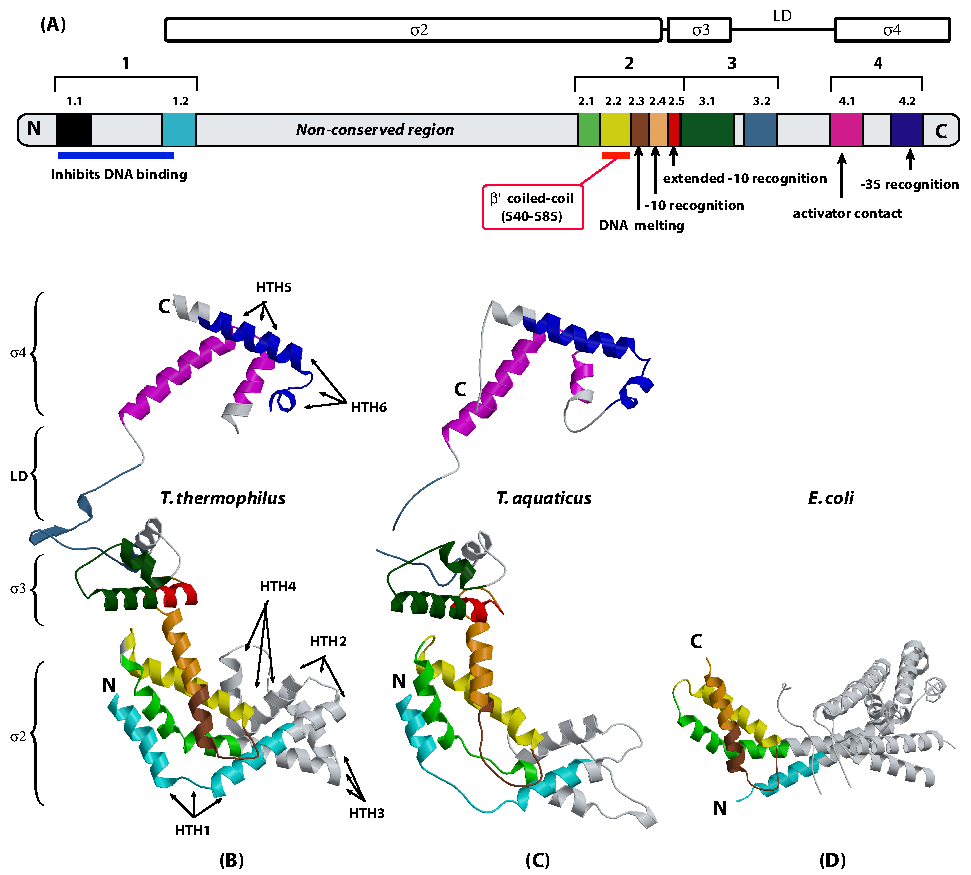
\includegraphics{figures/chap1_sigma_structure}
\end{narrow}
\caption[$\sigmaup$ structure-function relationship]{$\sigmaup$
structure-function relationship. \textbf{(A)} The four conserved
regions of $\sigmaup$\smallsu{70} factors shown color-coded. The
function of each region is indicated by arrow. The regions of
major interaction with core RNA polymerase is indicated by red
line. The box representation on top indicates the three protease
resistant domains of $\sigmaup$, connected by the linker domain
(LD). \textbf{(B)} The crystal structure of $\sigmaup$ factor of
\emph{T. thermophilus}~\citep{Vassy2002}, when bound to
holoenzyme. The six helix-turn-helix (HTH) domains are labelled.
Drawn using the extracted coordinates of only $\sigmaup$ from the
coordinates of the holoenzyme (1IW7). \textbf{(C)} The crystal
structure of \emph{T. aquaticus} $\sigmaup$ as in
holoenzyme~\citep{Murakami2002b}. Drawn using the extracted
coordinates of only $\sigmaup$ from the coordinates of the
holoenzyme (1L9U). \textbf{(D)} The crystal structure of the
\emph{E. coli} $\sigmaup$\smallsu{70} fragment from region
1.2--2.4~\citep{Malhotra1996}. Drawn from PDB entry 1SIG. (B),
(C), and (D) are color-coded as in (A) and were drawn using
MolScript~\citep{Esnouf1997} and Raster3D~\citep{Merrit1997}.}

\label{chap1:sigma}
\end{figure}

Crystal structures and proteolysis data indicate that \s{} has
three compact domains: \s{}2, \s{}3, and
\s{}4~\citep[][Figure~\ref{chap1:sigma}A and B]
{Campbell2002,Murakami2002b,Vassy2002}. \s{}3 and \s{}4 are
connected by a flexible linker domain (LD). The structures also
revealed that \s{} is entirely composed of $\alphaup$ helices and
coils. The \s{}2 domain of \emph{Thermus} species contains eight
$\alphaup$ helices spanning region 1.2 through N-terminal half of
the region 2.4, which constitutes four helix-turn-helix motifs
(Figure~\ref{chap1:sigma}B). The \s{}3 domain spans regions
2.4--2.5 and 3.1 and consists of 3 $\alphaup$ helices. The LD
consists of 30 residues mostly from region 3.2 which from a
hairpin loop into the DNA main channel near the $\betaup'$
\emph{rudder} (Section~\ref{chap1:RNAP}). Domain \s{}3, which
contains regions 4.1 and 4.2, contains four $\alphaup$ helices
arranged as two helix-turn-helix motifs.


The crystal structure of \s{}2 fragment of \bact{Ec}
\siga{}~\citep{Malhotra1996} differs in the same region from
\emph{Thermus} in having 14 $\alphaup$ helices while \s{}2 of
\emph{Thermus} species only has 8 $\alphaup$ helices. The
difference comes from a nonconserved 175 amino acids insertion
between region 1.2 and 2.1 in \bact{Ec}, which is absent in
\emph{Thermus} species.  Except the difference in the nonconserved
helices \bact{Ec} and \emph{Thermus} \s{} are structurally
comparable as far as the orientation of the conserved region is
concerned (Figure~\ref{chap1:sigma}B, C, and D).

\subsubsection{Region 1.1}
\label{region1_1} The N-terminal region 1.1 of \s{} is largely
disordered and no structural information is available, as all the
crystallized \s{} factors till date lacks conserved region 1.1
(Figure~\ref{chap1:sigma}B, C and D). This domain is thought to be
self-inhibitory, which is known to mask the DNA-binding regions of
\s{} before it binds to the core~\citep{Dombroski1993}.
Fluorescence Resonance Energy Transfer (FRET) analysis locates
region 1.1 in the downstream of the DNA channel in holoenzyme.
During open complex formation this region comes out the DNA
channel~\citep{Mekler2002}. It has been proposed that this region
plays a crucial role in the open complex formation by means of
opening the two pincers of the RNAP which is a rate limiting step
in transcription initiation~\citep{Young2002}. This region is
present only in primary \s{}. It is therefore, remains to be seen
how alternative \s{} factors perform this function.

\subsubsection{Core-binding}
\label{chap1:core_binding} Crystal structure of RNAP holoenzyme
revealed extensive contact of \s{} with the core RNAP, which
confirms the genetic studies~\citep{Sharp1999}. The total contact
area (\U{$\sim$8200}{\AA}) is usually large, and is comparable to
largest contact areas of oligomeric
proteins~\citep{Murakami2002b}. The primary interface (red line in
Figure~\ref{chap1:sigma}A) involves region 2.2 and $\betaup'$
coiled-coiled region ($\betaup'$ 540--585), which corresponds well
with earlier binding studies and mutational analysis indicating
interaction of region 2.2 with $\betaup'$
coiled-coil~\citep{Sharp1999,Arthur2000,Joo1997,Young2001}.

\mathversion{bold}
\subsubsection{$-$10 binding and melting}
\mathversion{normal}

\label{chap1:melting} A number of studies using a variety of
primary and alternative \s{} factors from \bact{Ec} and \emph{B.
subtilis} have identified site-specific mutations in region 2.4
that suppress single-base mutations within the $-$10 promoter
element. All these studies converge on the conclusion that Q437
and T440 (numbers indicate \bact{Ec} \siga{} amino acid positions)
suppress specific base changes at T($-$12) of
\su{$-$12}TATAAT\su{$-$7}. The spacing of these residues and
absolutely conserved hydrophobic amino acid residues at position
435, 439, and 443 led to the proposal that region 2.4 of \s{}
forms an amphipathic $\alphaup$ helix with Q437 and T440 of \s{}
contacting T($-$12) of promoter, and R441 contacts $-$13 base of
the
promoter~\citep{Siegele1989,Kenny1989,Daniels1990,Waldburger1990}.
Region 2.4 is indeed amphipathic $\alphaup$ helix in \bact{Ec} and
\emph{Thermus} species. Moreover, in the crystal-structure of
holoenzyme and fork-DNA complex from \emph{T. aquaticus}, this
region was found to contact the major groove of the DNA, and the
amino acids corresponding to \bact{Ec} \s{} were all in the
vicinity of $-$10, thus confirming the earlier conclusions.

In region 2.5, (recently renamed as region 3.0) two residues H455
and E458 of \bact{Ec} \siga{} was critical for recognizing
\emph{extended $-$10} element~\citep{Barne1997}. E458 was shown to
be critical for recognition of extended $-$10, whereas, H455
appears to play a non-specific DNA binding role. For \bact{Ec}
\sigs{}, K173 (corresponding to E458 of \siga{}) is shown to
interact directly with C($-$13) of \sigs{}-controlled
promoters~\citep{Becker2001}. In the crystal structure of \emph{T.
aquaticus}, H278 (corresponding to H455 of \bact{Ec}) is found to
be too far away to contact extended $-$10 base. Its role thus
remain unclear.

A large body of data implicates the conserved basic and aromatic
residues of \s{} in region 2.3 help in the nucleation of the
strand separation, possibly by base flipping  of A($-$11) of
promoters~\citep{Helmann1999,Panaghie2000,Fenton2000,Tomsic2001}.
It has been suggested that the strand opening is initiated by
stacking of A($-$11) between Y430 and W433 of \bact{Ec} \siga{}
while K414 and K418 possibly stabilizes the resulting separated
strands~\citep{Tomsic2001,Tsu2002}. In crystal structure of
\emph{T. aquaticus} the nontemplate strand of the promoter indeed
drapes over residues corresponding to these residues in \bact{Ec}.

\mathversion{bold}
\subsubsection{$-$35 recognition}
\mathversion{normal}

In addition to region 2, region 4 is the most conserved region in
the \siga{} family~\citep{Lonetto1992}. Genetic studies indicated
that the residues from region 4.2 determine sequence-specific
interaction with the $-$35
element~\citep{Gradella1989,Kenney1991,Siegele1989}. The crystal
structure of the region 4 of \emph{T. aquaticus} \s{} with $-35$
element confirmed the above conclusion~\citep{Campbell2002}. Two
residues of region 4.1 and nine residues from region 4.2 directly
or indirectly interacts with \su{$-$35}T\-T\-G\-A\-C\-A\su{$-$30}
sequence with R584 (\bact{Ec} numbering) contacting G($-$31) (on
the template strand) by two hydrogen bonds, E585 contacting
C($-$33) with one hydrogen bonds, and Q589 contacting T($-$35) (on
nontemplate strand) with one hydrogen bond.

\mathversion{bold} \subsubsection{$-$35 contact in dispensable}
\mathversion{normal}

The contact at $-35$ is not essential for transcription from all
the promoters. For example, region 4 of \siga{} is dispensable for
promoters containing an \emph{extended $-$10}
element~\citep[\textbf{TG}nTATAAT;
][]{Barne1997,Keilty1987,Kumar1993,Campbell2002}. It might be
recalled that \emph{extended $-$10} makes contact with region
2.5(3.0) of \s{}\@. In fact, very recently, after elucidation of
the crystal structure of \emph{T. aquaticus} RNA polymerase,
\citet{Campbell2002} have claimed that the region 1.2--3.1 of \s{}
contains all the elements that are required for its function.
Region 4 is necessary for decreasing the K\sub{m} for the
substrates of the holoenzyme.

Moreover, experiments carried out with \emph{fic} promoter, which
does not use -35 contact at all~\citep{Tanaka1995}, and with point
mutations isolated in \emph{osmE} promoter~\citep{Bordes2000} as
well as compilations of promoter sequences from \bact{Ec}
\citep{Espinosa1996} indicate that the promoters recognized by
alternative \s{} factor \sigs{} have weak or no $-$35 region
specificity~\citep{Becker2001}. Recognition of $-$35 element is,
therefore, of less importance for \sigs{}.

\mathversion{bold}
\section{Classification $\sigmaup$-factors}
\mathversion{normal} \label{sig_class} Based on the sequence
similarity, the bacterial $\sigmaup$-factors can be grouped into
two families, the \siga{}- and $\sigmaup$\su{54}-family
(Table~\ref{sigma_classification}). The names were derived from
the \U{70}{kDa} primary $\sigmaup$-factor and \U{54}{kDa} nitrogen
regulator $\sigmaup$ factor of \bact{Ec}. These two groups of
$\sigmaup$ factor differs in their sequence and in their mode of
action. For example, while free \siga{} family member cannot bind
to the promoter without the core enzyme, $\sigmaup$\su{54} members
can bind to promoter without the core enzyme~\citep{Ishihama1993}.
Additionally, \s\su{54} requires energy from the hydrolysis of ATP
by an activator protein for promoter
activation~\citep{Merrick1993}.


\begin{table}[tbp]
\linespread{1}\normalsize
\renewcommand{\arraystretch}{1.5}
\begin{minipage}[c]{\textwidth}
\renewcommand{\footnoterule}{}
\renewcommand{\footnotesep}{0pt}
\caption[Eubacterial $\sigmaup$ factors]{$\sigmaup$ factors of
pseudomonads and Enterobacteriaceae and related $\sigmaup$ factors
from other bacteria.
After~\citet{Lonetto1996,Wosten1998,Lonetto1992}.}
\label{sigma_classification}
\begin{narrow}{-1in}{-1in}
\centering
\begin{small}
\begin{tabularx}{6.1in}{@{}>{\raggedright\arraybackslash}p{1in}>{\raggedright\arraybackslash}p{.5in}>{\raggedright\arraybackslash}X>{\raggedright\arraybackslash}X@{}}\toprule

\textbf{Class} & \textbf{Gene}\protect\footnote{as in pseudomonads
and Enterobacteriaceae.}& \textbf{Related $\sigmaup$ factor} &
\textbf{Function}\\\midrule
\multicolumn{4}{c}{\textbf{$\sigmaup$\smallsu{70}-family Group 1:
Primary sigma factors}}\\ Primary $\sigmaup$-factors & \emph{rpoD}
& Gram-negative bacteria, $\sigmaup$\smallsu{70},
$\sigmaup$\smallsu{D}; Gram-positive bacteria
$\sigmaup$\smallsu{A}; Mycobacteria, MysA; Streptomyces, HrdB &
Major $\sigmaup$ factor during exponential growth
\\

\multicolumn{4}{c}{\textbf{$\sigmaup$\smallsu{70}-family
Group~2:~Non-essential primary-like $\sigmaup$ factors}}
\\


Stationary phase $\sigmaup$-factor& \emph{rpoS} &
$\sigmaup$\smallsu{S}, $\sigmaup$\smallsu{38} in pseudomonads and
Enterobacteriaceae & Major $\sigmaup$-factor during stationary
phase; response to several stress conditions\\

 Cyanobacterial $\sigmaup$-factors & --- & \emph{Synechococcus},
\emph{Synechocystis}, \emph{Anabaena}, SigB--E & Controlling gene
expression during circadian responses, carbon and nitrogen
availability or post-exponential growth phase\\

$\sigmaup$-factors of Gram-positive high-GC bacteria & --- &
\emph{Mycobacteria}, MysB; \emph{Corynebacteria}, SigB;
Streptomyces, HrdA, HrdC--E & Unknown\\

\multicolumn{4}{c}{\textbf{$\sigmaup$\smallsu{70}-family Group 3:
Alternative $\sigmaup$ factors}}
\\
$\sigmaup$\smallsu{32} related & \emph{rpoH}, \emph{htpR} &
Gram-negative bacteria $\sigmaup$\smallsu{H}
($\sigmaup$\smallsu{32}); \emph{Citrobacter}, HtpR;
\emph{Myxococcus xanthus}, $\sigmaup$\smallsu{B} & Transcription
of heat-shock proteins, fruiting body formation\\

$\sigmaup$\smallsu{B} related & --- & \emph{Bacillus},
\emph{Staphylococcus}, $\sigmaup$\smallsu{B}; \emph{Mycobacteria},
\emph{Streptomyces}, $\sigmaup$\smallsu{F} & Gene expression
during stress or late sporulation \\

Flagellar $\sigmaup$-factor & \emph{fliA}, \emph{flaD} &
Enterobacteriaceae $\sigmaup$\smallsu{F} ($\sigmaup$\smallsu{28});
\emph{Bacillus}, $\sigmaup$\smallsu{D}; \emph{Streptomyces}, WhiG
& Late flagellar gene expression and early sporulation
\\

ECF $\sigmaup$-factor & \emph{rpoE} (\emph{E. coli}) & \emph{P.
aeruginosa}, AlgU (AlgT); \emph{E. coli}, Mycobacteria,
\emph{Photobacterium}, $\sigmaup$\smallsu{E}; \emph{P. syringae}
HrpL & Alginate biosynthesis, antibiotic production, response to
periplasmic stress, extreme heat-shock \\

Metal transport $\sigmaup$ factor & \emph{fecI} (\emph{E. coli}) &
\emph{P. putida}, PupI; \emph{P aeruginosa}, \emph{P.
fluorescens}, PvdS; \emph{Bacillus}, $\sigmaup$\smallsu{X};
\emph{Alcaligenes}, NccH, CnrH & Iron citrate transport (\emph{E.
coli}), siderophore regulation (\emph{Pseudomonas}), nickel and
cobalt resistance \\

Sporulation $\sigmaup$-factors & --- & \emph{Bacillus},
\emph{Clostridium}, $\sigmaup$\smallsu{E}, $\sigmaup$\smallsu{F},
$\sigmaup$\smallsu{G}, $\sigmaup$\smallsu{H},
$\sigmaup$\smallsu{K} & Expression of sporulation genes
\\

\multicolumn{4}{c}{\textbf{$\sigmaup$\smallsu{54}-family}}
\\

$\sigmaup$\smallsu{N} related & \emph{rpoN}, \emph{ntrA},
\emph{glnF} & $\sigmaup$\smallsu{54}, $\sigmaup$\smallsu{55},
$\sigmaup$\smallsu{N} from various species; \emph{Bacillus},
$\sigmaup$\smallsu{L} & Nitrogen metabolism, formate degradation,
phage shock response, levansucrase regulation in
\emph{Bacillus}\\\bottomrule

\end{tabularx}
\end{small}
\end{narrow}
\end{minipage}
\renewcommand{\arraystretch}{1.0}
\linespread{1.1}\normalsize
\end{table}

The \siga{}-family can be further divided into three different
functionally and structurally related groups~\citep[][
Table~\ref{sigma_classification}]{Lonetto1992}:

\begin{description}

\item[Group 1] consists of the house-keeping $\sigmaup$-factor,
responsible for the majority of the transcription during
exponential growth. The classes of $\sigmaup$-factors are
essential for the viability of the cells. All primary $\sigmaup$
factors from diverse bacteria fall into this class.

\item[Group 2] consists of the $\sigmaup$ factors very similar to
Group 1, but they are non-essential for cell survival. The best
example is \emph{rpoS} of \bact{Ec} and pseudomonads.

\item[Group 3] consists of $\sigmaup$ factors under the \siga{}
family, but quite divergent from the Group 1, exhibiting only 27\%
identity with the primary $\sigmaup$-factors. Members of this
subgroup are more similar among themselves than to the Group 1
$\sigmaup$-factors of the same species. For example, the
heat-shock $\sigmaup$-factor from \emph{Citrobacter}, HtpR, is
94\% identical to RpoH of \bact{Ec}, whereas, \bact{Ec} primary
$\sigmaup$ has only 24\% identity with \bact{Ec} RpoH. This type
of low similarity suggests a possible convergent
evolution~\citep{Lonetto1992}.

\end{description}

In \bact{Ec}, belonging to $\gammaup$ proteobacteria superfamily,
there are seven \s{} factors~\citep{Ishihama2000}. All these seven
\s{} factors and their homologs from other species and their
functions are listed in Table~\ref{sigma_classification}. Till
date, the only pseudomonad genome, which is sequenced, is of
\bact{Pa}~\citep{Stover2000}. A search in the genome annotation
(\seq{www.pseu\-do\-monas.com}) revealed 24 putative \s{}-factors
(Table~\ref{aeruginosa_sig}). It is to be noted that there are 17
putative ECF family \s{}-factors in the \bact{Pa} genome.

\begin{table}[tbp]
\linespread{1}\normalsize
\renewcommand{\arraystretch}{1.4}
\begin{minipage}[c]{\textwidth}
\renewcommand{\footnoterule}{}
\renewcommand{\footnotesep}{0pt}
\caption[\s{}-factors in \bact{Pa} genome]{\s{}-factors in
\bact{Pa} genome} \label{aeruginosa_sig}
\begin{narrow}{-1in}{-1in}
\centering
\begin{small}
\begin{tabularx}{5.5in}{%
@{}>{\raggedright\arraybackslash}X%
>{\raggedright\arraybackslash}p{2.2in}%
>{\raggedright\arraybackslash}X%
>{\raggedright\arraybackslash}X%
>{\raggedright\arraybackslash}X@{}}\toprule

  \textbf{PaNumber}\protect\footnote{\bact{Pa} database accession number} & \textbf{Protein name} & \textbf{Gene name} &  \textbf{From (bp)} &   \textbf{To (bp)}
  \\\midrule

    PA0576 & RpoD (\s\smallsu{D}) &       \emph{rpoD} &     636224 &     634371 \\

    PA3622 & RpoS (\s\smallsu{S}) &       \emph{rpoS} &    4058912 &    4057908 \\

    PA0376 & RpoH (\s\smallsu{H}) &       \emph{rpoH} &     420683 &     421537 \\

    PA1455 & FliA &       \emph{fliA} &    1584795 &    1585538 \\

    PA2426 & PvdS &       \emph{pvdS} &    2722174 &    2722737 \\

    PA0762 & AlgU & \emph{algU} (\emph{algT}) &     831301 &     831882 \\

    PA0149 & probable, ECF subfamily &            &     169361 &     169906 \\

    PA0472 & probable, ECF subfamily &            &     534027 &     533509 \\

    PA0675 & probable, ECF subfamily &            &     734872 &     735417 \\

    PA1300 & probable, ECF subfamily &            &    1409949 &    1410476 \\

    PA1351 & probable, ECF subfamily &            &    1464878 &    1466101 \\

    PA1363 & probable, ECF subfamily &            &    1474727 &    1475467 \\

    PA1776 & probable, ECF subfamily &            &    1920568 &    1921065 \\

    PA1912 & probable, ECF subfamily &            &    2085929 &    2085423 \\

    PA2050 & probable, ECF subfamily &            &    2244492 &    2244998 \\

    PA2093 & probable, ECF subfamily &            &    2304318 &    2304827 \\

    PA2387 & probable, ECF subfamily &            &    2640871 &    2640392 \\

    PA2468 & probable, ECF subfamily &            &    2786882 &    2786364 \\

    PA2896 & probable, ECF subfamily &            &    3251321 &    3250737 \\

    PA3285 & probable, ECF subfamily &            &    3678330 &    3677719 \\

    PA3410 & probable, ECF subfamily &            &    3819111 &    3818596 \\

    PA3899 & probable, ECF subfamily &            &    4367282 &    4367791 \\

    PA4896 & probable, ECF subfamily &            &    5491180 &    5490644 \\

    PA4462 & \s\smallsu{54} &       \emph{rpoN} &    4992869 &    4994362
    \\\bottomrule

\end{tabularx}
\end{small}
\end{narrow}
\end{minipage}
\linespread{1.1}\normalsize\renewcommand{\arraystretch}{1}
\end{table}

All these discrete families of \s{}-factors directs the RNA
polymerase to transcribe from discrete set of promoters. Consensus
promoter sequence for each of these \s{}-factors, except the
sporulation \s{}-factors in \emph{Bacillus}, is shown in
Table~\ref{sigma_promoters}.

\begin{table}[tbp]
\linespread{1}\normalsize
\renewcommand{\arraystretch}{1.4}
\begin{minipage}[c]{\textwidth}
\renewcommand{\footnoterule}{}
\renewcommand{\footnotesep}{0pt}
\caption[Consensus promoters of known \s{} factors]{Consensus
promoters of the known \s{} factors\protect\footnote{except the
sporulation \s-factors of \emph{Bacillus}}.}
\label{sigma_promoters}
\begin{narrow}{-1in}{-1in}
\centering
\begin{small}
\begin{tabularx}{6.1in}{%
@{}>{\raggedright\arraybackslash}p{1in}%
>{\raggedright\arraybackslash}X%
>{\raggedright\arraybackslash}X%
>{\raggedright\arraybackslash}X%
>{\raggedright\arraybackslash}X%
>{\raggedright\arraybackslash}p{1.5in}@{}}\toprule

\textbf{$\sigmaup$\ class} & \textbf{Name} & \textbf{$-$35} &
Spacer & \textbf{$-$10} & \textbf{References} \\\midrule

Primary $\sigmaup$-factors & RpoD, SigA & TTGACA & 16--18 &
TATAAT & \citet{Harley1987,Helmann1995}\\

Stationary phase $\sigmaup$-factors & RpoS & -- & -- &
CTATACT & \citet{Espinosa1996} \\

Heat-shock $\sigmaup$ ($\sigmaup$\su{32}) factor & RpoH  &
CTTGAAA &11--16& CCCATnT & \citet{Gross1996}\\

& SigB & GTTTAA & 12--14 & GGGTAT &
\citet{Hecker1996}\\

Flagellar $\sigmaup$-factor & $\sigmaup$\smallsu{28}, FliA, SigD &
TAAA & 15 & GCCGATAA &
\citet{Helmann1991}\\

ECF $\sigmaup$-factors & RpoE, SigE & GAACTT & 16--17 & TCTRA &
\citet{Lonetto1994,Martin1994,Raina1995,Rouviere1995}\\

\s\su{54}-family & RpoN, SigL & TGGCAC & 5 & TTGCW &
\citet{Merrick1993} \\\bottomrule
\end{tabularx}
\end{small}
\end{narrow}
\end{minipage}
\linespread{1.1}\normalsize \renewcommand{\arraystretch}{1}
\end{table}

\mathversion{bold}
\section{A note about the nomenclature of \s{} factors}
\mathversion{normal}

There are considerable confusions over the naming of $\sigmaup$
factors~\citep{Lonetto1996}. A scanning of the literature,
however, indicates that a consensus is gradually emerging. The
Gram-negative bacterial $\sigmaup$-factors are named,
consistently, after the names given in \bact{Ec}. For example,
\emph{Pseudomonas} primary $\sigmaup$ factors is called as
\s\su{D} or RpoD and the gene is called as \emph{rpoD}. The
Gram-positive bacterial $\sigmaup$-factors, on the other hand, are
named with superscripted alphabets in capitals, and the
corresponding genes are named as \emph{sig}$\ast$, where
``$\ast$'' denotes an alphabet. \emph{Bacillus} primary
$\sigmaup$-factor is called $\sigmaup$\su{A} or SigA and the
corresponding gene is named as \emph{sigA}. Note that conflicting
naming scheme sometimes arise. For example, primary
$\sigmaup$-factor, \siga{} in \bact{Ec}, is also called
$\sigmaup$\su{D} which is no way similar to \emph{Bacillus}
$\sigmaup$\su{D}.

In this thesis, the primary and the stationary phase
$\sigmaup$-factor of Lz4W will be called with their corresponding
names in \bact{Ec}. The primary $\sigmaup$-factor of Lz4W will be
called as, \s\su{D} or RpoD, and the corresponding gene will be
called as \emph{rpoD}, or sometimes as \emph{rpoD}\sub{Lz4W}. The
stationary phase $\sigmaup$ factor will be called as, \sigs{} or
RpoS, and the corresponding gene will be called as \emph{rpoS} or
sometimes as \lzsig{}.

\mathversion{bold}
\section{$\sigmaup$\su{S}---the master regulator of stress-response}
\mathversion{normal}


\begin{table}[tbp]
\linespread{1}\normalsize
\renewcommand{\arraystretch}{1.5}
\begin{minipage}[c]{\textwidth}
\renewcommand{\footnoterule}{}
\renewcommand{\footnotesep}{0pt}
\caption[\sigs{} controlled genes]{Repertoire of \sigs{}
functions. Only a very limited set of genes is shown. After
\citet{Hengge1996,Loewen1994,Ishihama2000}.}
\label{chap1:rpos_genes}
\begin{narrow}{-1in}{-1in}
\centering
\begin{small}
\begin{tabularx}{5.5in}{%
@{}>{\raggedright\arraybackslash}X%
>{\raggedright\arraybackslash}p{3.9in}@{}}\toprule
\textbf{Function} & \textbf{Examples}\\\midrule Prevention and
repair of DNA damage & $\sim$16 genes; \e{katE} and \e{kaG},
encoding catalases
HPII and HPI; \e{xthA}, encoding exonuclease III; \e{dps}, a DNA binding protein; \e{aidB}, invloved in repairing methylation damage to DNA \\

Cell morphology and division & $\sim$20 genes;\e{bolA}, a
morphogen; \e{fic}, involved in cell division; \e{ftsAQZ}, septum formation \\

Membrane and cell envelope functions & \e{osmB}, lipoprotein
involved in cell surface alteration; \e{osmY}, capsule formation;
\e{cfa}, cyclopropane fatty acid synthase \\

Modulation of virulence genes & \e{spvA}, a virulence factor; \e{csgA}, curli formation \\

Osmoprotection and thermotolerance & \e{otsBA}, trehalose
synthesis; \e{htrE}, function unknown\\

Glycogen synthesis & \e{glgS} \\

Anaerobically induced genes & \e{appY}, regulatory protein;
\e{appCB}, cytochrome oxidase, \e{hyaABCDEF}, hydrogenase I;
\e{appA}, acid phosphatase \\

Energy metabolism and anabolism & $\sim$15 genes; \e{acs},
Acetyl-CoA synthetase; \e{frd}, fumarate reductase \\

DNA replication & \e{dnaN}, DNA polymerase III $\betaup$-subunit;
\e{topA}, DNA topoisomerase I \\

\bottomrule
\end{tabularx}
\end{small}
\end{narrow}
\end{minipage}
\linespread{1.1}\normalsize \renewcommand{\arraystretch}{1}
\end{table}


\sigs{} is a subunit of RNAP in Gram-negative bacteria, that is
induced and can partially replace the vegetative \s{} factor under
many stress conditions and at stationary phase . As a consequence,
transcription of numerous \sigs{}-dependent genes are
activated~\citep[reviewed
in][Table~\ref{chap1:rpos_genes}]{Loewen1994,Hengge1996,Ishihama2000}.
In \bact{Ec}, several groups had identified \e{rpoS} independently
for different phenotypes, and named accordingly. The gene was thus
named as \e{nur}, \e{katF}, \e{appR}, \e{csi-2}, and \e{abrD} and
finally \e{rpoS}, depending on the context in which it was
discovered. Soon it was realized that all these phenotypes were
because of the mutation in the same gene which resulted in a
pleiotropic phenotype with a rapid loss of viability under various
stress conditions, including near-UV exposure, high-salt, hydrogen
peroxide, elevated temperature, low pH and prolonged
starvation~\citep{Loewen1994,Hengge2002,Hengge1996}. In other
Gram-negative bacteria, \e{rpoS} functions in a manner, similar to
that of \bact{Ec} except some minor differences.




In \bact{Ec} K12 genome~\citep{Blattner1997}, \e{rpoS} is present
at 61.747 centisome, from 2,865,574 to 2,864,582 bp of the
chromosomal DNA, on the complementary strand. In \bact{Pa}
genome~\citep{Stover2000} the gene is present at 64.777 centisome
from 4,058,912 to 4,057,908 bp on the complementary strand.

\section{Regulation of \emph{rpoS} expression}
The genes under \e{rpoS} regulation is primarily modulated by the
level of expression of \e{rpoS} itself. The cellular \sigs{} level
increases in response to starvation for carbon, nitrogen,
phosphate, and amino acids, which mark the entry of the cells into
stationary phase. \sigs{} level can also be induced by several
other conditions, such as, reduction of the growth
rate~\citep{Gentry1993,Jishage1995,Jishage1996,Lange1991,Lange1994,Notley1996},
high cell density~\citep{Lange1994}, low pH~\citep{Bearson1996},
hyperosmolarity~\citep{Muffler1996}, high
temperature~\citep{Muffler1997}, low
temperature~\citep{Sledjeski1996} and even magnetic
field~\citep{Tsuchiya1999}. All these stressors affect \emph{rpoS}
expression at various levels-- transcription, translation as well
as post-translation. This is shown graphically in
Figure~\ref{intro_rpos_control}. The major factors affecting
\emph{rpoS} expression are discussed below, with special emphasis
on \emph{rpoS} expression during growth at low temperature. For
details see recent reviews by \citet{Hengge2002b,Hengge2002}.

\begin{figure}[tbp]
\begin{narrow}{-1in}{-1in}
\centering
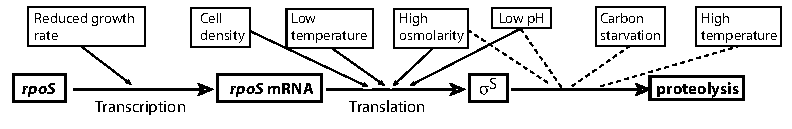
\includegraphics{figures/chap1_rpos_control}
\end{narrow}
\caption[Regulation of \emph{rpoS} expression]{Regulation of
\emph{rpoS} expression by various stressors. The solid arrow
indicates activation and dotted line indicates repression. Redrawn
from \citet{Hengge2002}.} \label{intro_rpos_control}
\end{figure}


\subsection{\emph{rpoS} promoter structure}

In majority of the gram negative bacteria, including \bact{Ec} and
pseudomonads, \emph{rpoS} is always linked with upstream
\emph{nlpD}, coding for a lipoprotein of unknown
function~\citep{Ichikawa1994,Lange1994b}. Downstream of
\emph{rpoS} is variable, even within \bact{Ec}
strains~\citep{Brown2001,Herbelin2000}.

In \bact{Ec}, two independent studies identified three different
transcription start sites of \emph{rpoS} mRNA within \emph{nlpD}
gene~\citep{Lange1995,Takayanagi1994}. Both these studies detected
only one common \e{rpoS} start site within \e{nlpD} (labelled
\e{rpoSp} in Figure~\ref{chap1:rpos_promoter}). This site is now
considered to be the major transcription start site of
\e{rpoS}~\citep{Hengge2002}. Transcription starts with a
T~\citep{Takayanagi1994} or G~\citep{Lange1995} located around
\U{567}{bp} upstream of \e{rpoS} start codon. The $-$10 element
(TATTCT) and $-$35 element (TTGCGT) resemble \siga{} consensus
sequence. These promoter elements are flanked by two cAMP-CRP
binding sites. Although, two upstream \e{nlpD} promoters (marked
\e{nlpDp1} and \e{nlpDp2} in Figure~\ref{chap1:rpos_promoter}) can
contribute to the basal level expression of \e{rpoS} but the
stationary phase expression of \e{rpoS} is solely driven by
\e{rpoSp}~\citep{Lange1995,Takayanagi1994}.

In \e{Pseudomonas}, the start site of the \emph{rpoS} mRNA was
located 366~\citep{Tanaka1994} to 371~\citep{Kojic2002} bases
upstream of the translation initiation codon. The sequences TTGAAT
and TCAATT, separated by 20 bases were found as potential $-35$
and $-10$ promoter elements. An additional observation was the
presence of a binding site of the regulatory protein, \e{psrA}
(see Section~\ref{chap1:psra}) in $-$35 region of the promoters.


\begin{figure}[tbp]
\begin{narrow}{-1in}{-1in}
\centering
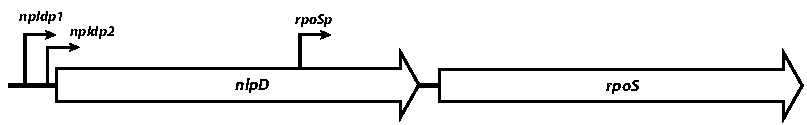
\includegraphics{figures/chap1_rpos_promoter}
\end{narrow}
\caption[Distribution of \emph{rpoS} promoters]{Distribution of
\emph{rpoS} promoters.  \emph{rpoSp} is the major \emph{rpoS}
promoter in \emph{E. coli} and the only promoter contributing to
\emph{rpoS} expression in pseudomonads. The position of \e{rpoSp}
in \bact{Ec} (\U{567}{bp} upstream from ATG codon) is different
from the position in pseudomonads (\U{$\sim$370}{bp} upstream from
the ATG codon). Genes are indicated by open arrows showing the
direction. Angled arrows represent the transcription start site.}
\label{chap1:rpos_promoter}
\end{figure}


\subsection{Transcriptional regulation of \emph{rpoS}}

In \bact{Ec}, \emph{rpoS} is mainly regulated by
post-transcriptional mechanism. Although, \e{rpoS} mRNA is present
in high-level, the level of \sigs{} protein is very low during
exponential phase, and mRNA level do not generally change under
stress conditions~\citep{Hengge2002}. Nevertheless, \e{rpoS} mRNA
increases almost five folds during slow growth in rich medium, and
during entry into stationary
phase~\citep{Lange1991,Lange1994,McCann1993,Mulvey1990,Schellhorn1992,Takayanagi1994}.

Several factors have been shown to regulate \e{rpoS}
transcription. Most of the studies had been carried out using
\e{rpoS}::\e{lacZ} transcriptional fusion. A summary of the
presently known key regulators of \e{rpoS} transcription is
presented in Table~\ref{rpos_trans_regulator}.

\begin{table}[tbp]
\linespread{1}\normalsize
\renewcommand{\arraystretch}{1.3}
\begin{minipage}[c]{\textwidth}
\renewcommand{\footnoterule}{}
\renewcommand{\footnotesep}{0pt}
\caption[Regualtors of \e{rpoS} transcription]{Regulators of
\e{rpoS} transcription} \label{rpos_trans_regulator}
\begin{narrow}{-1in}{-1in}
\centering
\begin{small}
\begin{tabularx}{6.1in}{%
@{}>{\raggedright\arraybackslash}p{.9in}%
>{\raggedright\arraybackslash}X%
>{\raggedright\arraybackslash}p{2.5in}%
>{\raggedright\arraybackslash}p{1.9in}@{}}\toprule

\textbf{Regulator} & \textbf{Type}\protect\footnotemark[1] &
\textbf{Observation} & \textbf{Reference}\\\midrule cAMP-CRP &
$+/-$ & \e{rpoS}::\e{lacZ} fusion expression high or low in
different \e{cya} mutant; high in
\e{crp} mutant & \citet{Lange1991,Lange1994,McCann1993}\\
\e{crr} & $-$ & Mutation elevates \e{rpos}::{lacZ} expression
through adenylate cyclase & \cite{Ueguchi2001}\\

Polyamines & $+$ & By stimulating adenylate cyclase expression
which affects RpoS level by positive effect through cAMP-CRP &
\citet{Yoshida2001}\\

GacS-GacA\protect\footnotemark[2] two-component system & $+$ &
Mutations causes more than 80\% reduction in RpoS protein level
and
\e{rpoS}::\e{lacZ} expression & ~\citet{Whistler1998}\\

BarA& $+$ & GacS homolog of \bact{Ec}; mutation decreases \e{rpoS}
mRNA level during exponential phase & \citet{Mukho2000} \\

PsrA\protect\footnotemark[2] & $+$ & A TetR family regulator;
directly induces \e{rpoS} expression binding to its $-$35 element
& \citet{Kojic2001,Kojic2002} \\

Polyphosphate & $+$ & Mutation in \e{ppK}, the gene resposible for
polyphosphate synthesis decreases stationary phase survival;
expression of yeast exopolyphosphatase which depletes
polyphosphate in cell, decreases \e{rpoS}::\e{lacZ} fusion
expression &
\citet{Crooke1994,Rao1996,Shiba1997}\\

ppGpp & $+$ & \e{relA}, \e{spoT} double mutant show reduced level
of \s\smallsu{S}; level can be restored by stimulating ppGpp
accumulation; possibly affect transcriptional elongation rather
than initiation
& \citet{Gentry1993,Lange1995}\\

Quorum sensing molecules & ? & Culture supernatant from spent
growth medium (\e{i.e.}, already grown culture) was used to assay
\e{rpoS}::\e{lacZ} activity. Conflicting data makes it impossible
to draw any conclusion &
\citet{Mulvey1990,Garcia1996,Hengge2002} \\

Weak acids & $+$ & Benzoate increases \e{rpoS}::\e{lacZ}
expression; acetate showed induction in one study, and no effect
in another &
\citep{Mulvey1990,Schellhorn1992}\\

Cellular NADH/NAD\smallsu{$+$} ratio & $-$ & High
NADH/NAD\smallsu{$+$} ratio downregulates \e{rpoS} transcription
& \citet{Sevcik2001}\\

\bottomrule
\end{tabularx}
\end{small}
\end{narrow}
\footnotetext[1]{$+$ and $-$ indicates positive and negative
regulator, respectively. $+$/$-$ indicates both positive and
negative regulator\@. ? indicates no conclusion due to conflicting
reports.} \footnotetext[2]{In pseudomonads.}
\end{minipage}
\linespread{1.1}\normalsize
\renewcommand{\arraystretch}{1}

\end{table}


\subsection{Translational regulation of \emph{rpoS}}

\subsubsection{Regulation by Hfq}

Hfq (HF-I), a \U{11.2}{kDa} RNA-binding protein was first
identified as a host factor essential for phage Q$\betaup$
replication in \e{Ec}. Hfq is highly conserved, very abundant
protein and has been implicated in variety of RNA-mediated
events~\citep{Moller2002,Zhang2002}. There are several
gene-regulatory small RNAs (sRNA) which bind to
Hfq~\citep[reviewed in][]{Wassarman2002}. Interestingly, three of
Hfq binding sRNAs are also involved in \e{rpoS} regulation: OxyS,
DsrA and RprA (see below). Mutation in \e{hfq} has a pleiotropic
phenotype~\citep{Tsui1994}. Hfq stimulates the degradation of
\e{ompA}, \e{miaA}, \e{mutS}, and its own
mRNA~\citep{Tsui1997,Vytvytska1998,Vytvytska2000}. It is also
required for efficient translation of \e{rpoS}
mRNA~\citep{Brown1996,Muffler1996}.

Studies indicated that Hfq probably directly binds to \e{rpoS}
mRNA~\citep{Majdalani2001,Muffler1996b,Sledjeski2001,Zhang1998}. A
5$'$ deletion analysis of \e{rpoS} mRNA indicated that a region
far upstream to the translation initiation site is important for
Hfq action~\citep{Cunning1998}. Mutation in the translation
initiation region of \e{rpoS} mRNA, which potentially disrupts the
secondary structure resulted in increased \e{rpoS} translation and
reduced Hfq dependence~\citep{Brown1997}.

Hfq belongs to a family of proteins including Sm and Lsm, whose
members in higher organism are present in spliceosome and play
important role in mRNA processing~\citep{Moller2002,Zhang2002}.
Consistent to their role in spliceosome, Hfq, in similar manner,
was shown to form ternary complex with its cognate RNA and
regulatory sRNAs. This complex formation was demonstrated at least
in two cases: OxyS binding with \e{flhA} mRNA and Spot42 with
\e{galK} mRNA~\citep{Moller2002,Zhang2002}. It was, therefore,
proposed that Hfq might control \e{rpoS} activity in a similar
manner~\citep{Wassarman2002,Hengge2002}.

\subsubsection{Regulation by H-NS}

H-NS is an abundant histone-like protein shown to form
nucleoprotein complexes and acts as a repressor for a variety of
genes. StpA is a paralog of H-NS, which acts more as an RNA
chaperone. Both H-NS and StpA are known to form homo- and
hetero-oligomers~\citep[reviewed
in][]{Atlung1997,Dorman1999,Williams1997}. H-NS is also known to
be a cold-shock protein~\citep{Teana1991}.

H-NS mutant exhibits strongly increased RpoS level at all growth
stages \citep{Barth1995,Yamashino1995}, due to enhanced
translation of \e{rpoS} mRNA and suppression of RpoS
proteolysis~\citep{Yamashino1995}. The molecular mechanism of H-NS
mediated repression of RpoS expression is still unclear, but may
be indirect, as H-NS deficiency has no effect on \e{rpoS}
translation in \e{hfq} mutant background~\citep{Muffler1996}.
DsrA, a regulatory sRNA (see below) is also known to suppress
H-NS~\citep{Lease2000}. H-NS is also known to play an antagonistic
role with HU, another known regulator of
\e{rpoS}~\citep{Dri1992,Deighan2000,Painbeni1997}. It might also
be possible that H-NS modulates \e{rpoS} by affecting
HU~\citep{Hengge2002}.

\subsubsection{Regulation by HU}

HU is a major component of the bacterial nucleoid and also
participates in gene regulation, DNA recombination, and DNA
repair~\citep{Hengge2002}. Moreover, HU is required for optimum
survival during prolonged starvation \citep{Claret1997}. In
Enterobacteriaceae and Vibrionaceae, two subunits, HU$\alphaup$
and HU$\betaup$, encoded by \e{hupA} and \e{hupB}, respectively,
contribute to the formation of active HU
protein~\citep{Oberto2001}\@. \e{hupAB} mutant exhibits strongly
reduced RpoS level due to reduced translation of \e{rpoS}
mRNA~\citep{Balandina2001}. HU binds with high affinity to a 150
nucleotide fragment of \e{rpoS} mRNA spanning the translation
initiation region~\citep{Balandina2001}.

\subsubsection{Riboregulators in RpoS expression}
\label{chap1:srna} Recently, it is becoming clearer that
abundantly present small regulatory RNAs (sRNA) play a very vital
role in gene regulation~\citep[reviewed
in][]{Altuvia2000,Wassarman2002,Eddy2001}. Collectively termed as
\e{riboregulators}, three of these sRNAs had already been found to
have profound influence on \e{rpoS} expression. DsrA and RprA
promote \e{rpoS} translation and OxyS inhibits it. All these sRNAs
are known to bind to Hfq~\citep{Wassarman2002}.

DsrA was originally identified as a multicopy suppressor of
H-NS-mediated silencing of \e{rcsA} gene in
\bact{Ec}~\citep{Sledjeski1995} and later on found to be essential
for increased \e{rpoS} translation at low
temperature~\citep{Sledjeski1996}.

DsrA is a 87 nucleotide RNA that folds into a three stem-loop
structure~\citep[][Figure~\ref{chap1_dsra}]{Lease2000,Majdalani1998}.
The stem-loop 1 and the following single-stranded part of DsrA
(marked with solid line in Figure~\ref{chap1_dsra}) are
complementary to an upstream \e{antisense element} of \e{rpoS}
mRNA that is assumed to base pair with the translation initiation
region (see also Chapter 4). This suggests that DsrA functions by
an \e{anti-anti-sense} mechanism that disrupts the intramolecular
basepairing  in \e{rpoS}
mRNA~\citep{Lease2000,Lease1998,Majdalani1998,Lease2000b}. DsrA
plays only a minor role in \e{rpoS} translation in cells growing
at higher temperature, but becomes a major stimulating factor at
low temperature~\citep{Sledjeski1996}. This stimulation is due to
increased transcription of \e{dsrA}, and a six fold increase in
the stability of DsrA at low temperature~\citep{Repoila2001}. Hfq
stabilizes DsrA, as well as alters its secondary structure to
enable it to interact with \e{rpoS} mRNA~\citep{Sledjeski2001}.


\begin{figure}[tbp]
\centering
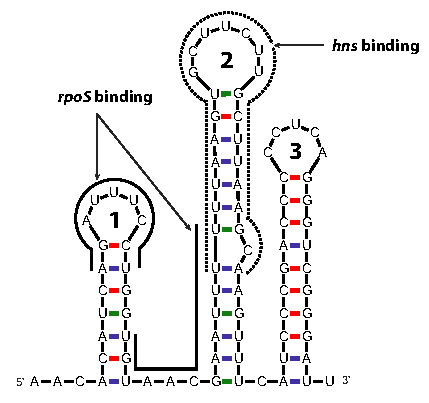
\includegraphics{figures/chap1_dsra}
\caption[DsrA sturcture]{DsrA RNA secondary structure. The lowest
energy structure predicted by MFOLD version
3.1~\citep{Mathews1999} is shown. The putative regions of \e{rpoS}
(solid line) and \e{hns} (dotted line) binding sites are
labelled.} \label{chap1_dsra}
\end{figure}

Besides directly regulating \e{rpoS}, DsrA negatively regulate
\e{hns} mRNA by formation of a coaxial stack with two regions of
\e{hns} mRNA by its unfolded stem-loop region 2
(Figure~\ref{chap1_dsra})\@. The \e{hns} mRNA is more efficiently
degraded within this complex~\citep{Lease2000b}. In what seems
like a reciprocal suppression, StpA and H-NS also represses
DsrA~\citep{Lease2000b}.

An indirect regulation of \e{rpoS} is also brought about by LeuO,
a LysR like regulator that binds to \e{dsrA}
promoter~\citep{Repoila2001} and represses its expression.
Overproduction of LeuO reduces \e{rpoS} translation in
DsrA-dependant manner particularly at low
temperature~\citep{Klauck1997}.

OxyS, a 109 nucleotide sRNA, which is induced by oxidative stress,
acts as a pleiotropic regulator~\citep{Altuvia1997}. A single
stranded A-rich region in OxyS RNA with no apparent sequence
complementarity with \e{rpoS}, is involved in the negative
regulation of \e{rpoS} translation~\citep{Zhang1998}. OxyS
coimmunoprecipitates Hfq, thus indicating that it might form a
translationally incompetent ternary complex with
\e{rpoS}~\citep{Zhang1998}.

Another sRNA involved in \e{rpoS} regulation is RprA, which was
identified as a multicopy suppressor for \e{dsrA}
mutation~\citep{Majdalani2001}. In presence of DsrA, neither
overproduction nor knockout of RprA has any effect on \e{rpoS}
expression.

\subsubsection{Other regulators}

There are several other regulators that have been shown to affect
RpoS expression at the level of translation. These regulators are
briefly described below.

\begin{description}

\item[\textbf{dnaK}] is a heat-shock chaperone\@. \e{dnaK} mutant
exhibits reduced \sigs{} level due to reduced \e{rpoS}
translation~\citep{Muffler1997,Rockabrand1998}.

\item[\textbf{DksA}] is zinc-binding protein. \e{dksA} mutation in
\e{Salmonella} exhibit reduced \sigs{} expression at stationary
phase and after a shift to acidic pH~\citep{Webb1999}.

\item[\textbf{EIIA(Glc)}] is negative regulator of \e{rpoS}
translation\@. In \e{crr} mutant which is defective in EIIA(Glc)
contains strongly elevated \sigs{}, which is suppressed by
external addition of cAMP~\citep{Ueguchi2001}.

\item[\textbf{CspC and CspE}] belongs to the cold shock protein
family in \bact{Ec}, although they are not cold-inducible.
Overproduction of these two RNA binding protein stabilizes
\e{rpoS} mRNA~\citep{Phadtare2001}.

\item[\textbf{UDP-glucose}] deficiency caused by mutation in
carbon-metabolism genes exhibits increased \sigs{} level during
exponential growth~\citep{Bohringer1995}.

\end{description}



\subsection{Control of \emph{rpoS} proteolysis}
\label{chap1_rssb}

In \bact{Ec}, \sigs{} level is low during exponential growth phase
due to its rapid degradation. Under stress conditions, the
proteolysis is prevented very quickly~\citep{Lange1994}. The
proteolysis is mediated by ATP-dependant ClpXP protease. Mutation
in the \e{clpP} and \e{clpX} results in stabilization of \sigs{}
\citep{Schweder1996}.

ClpXP can not degrade the \sigs{} alone. For this it requires a
recognition factor called RssB(SprE, MviA, ExpM in different
bacteria)~\citep{Muffler1996c,Hengge2002}. A mutation in \e{rssB}
stabilizes \sigs{}, resulting in elevated expression in
exponential phase~\citep{Muffler1996c}.

RssB is a response regulator of a two component pathway whose
cognate sensor kinase is yet unidentified. Acetyl phosphate is
known to play a role in RssB phosphorylation~\citep{Bouche1998}.
It is phosphorylated at its N-terminal domain at a conserved
aspartyl residue (D58)~\citep{Becker1999}. The phosphorylated form
directly binds to \sigs{} in equimolar ratio~\citep{Klauck2001}.
The binding involves K173 in region 2.5 of \sigs{}. A single point
mutation K173E was shown to stabilize \sigs{}~\citep{Becker1999}.
Once formed, the RssB-\sigs{} complex is recognized by ClpXP
protease and the \sigs{} is completely degraded in an
ATP-dependant manner.


\section{\emph{rpoS} in pseudomonads}
\index{rpoS@\emph{rpoS}!in pseudomonads}

A \emph{rpoS} homolog was cloned from Pseudomonads for the first
time in 1994, from \emph{P. aeruginosa}~\citep{Tanaka1994}. The
operon structure of \e{rpoS} was found to be similar to that of
\emph{E. coli}. The RpoS level was found to be higher at the onset
of stationary phase and the gene could restore the catalase
activity in \emph{rpoS}-deficient strain of \bact{Ec}. Strangely,
the same group in another article reported the inability of \emph{
P. aeruginosa rpoS} to get transcribed in \emph{E.
coli}~\citep{Fujita1994}. \emph{rpoS} was found to be transcribed
from its own promoter and the start site of the \emph{rpoS} mRNA
was located 366 bases upstream of translation initiation codon.
The sequences TTGAAT and TCAATT, separated by 20 bases were
identified as $-35$ and $-10$ elements of potential promoter. The
downstream region of the $-10$ sequence (GGGCCAGC) was found to be
similar to the ``gearbox'' sequence (CGGCAAGT).

Other studies on \emph{P. aeruginosa rpoS} indicated its role in
stationary-phase-specific stress resistance~\citep{Jorgensen1999}.
Interestingly, at stationary-phase \emph{rpoS}$^{-}$ cells were
much more stress resistant than \emph{rpoS}$^{+}$ cells from
exponential phase. Studies on \emph{P. aeruginosa} PAO1 also
showed that \emph{rpoS}$^{-}$ cells were sensitive to carbon
starvation only in medium containing glucose as carbon
source~\citep{Suh1999}. In addition, the \emph{rpoS} mutant of
PAO1 was hypersensitive to heat shock at 50\dg, increased
osmolarity, and prolonged exposure to high concentrations of
H$_{2}$O$_{2}$. Catalase production was also 60\% lower in these
mutants. The rpoS mutant produced 50\% less exotoxin A, but
produced only slightly smaller amounts of elastase and LasA
protease than the parent strain. The levels of phospholipase C and
casein-degrading proteases were also unaffected by a mutation in
\emph{rpoS} in PAO1. The rpoS mutation resulted in the increased
production of the phenazine antibiotic pyocyanin and the
siderophore pyoverdine. In an alginate-overproducing cystic
fibrosis (CF) isolate, FRD1, the \emph{rpoS101::aacCI} mutation
almost completely abolished the production of alginate when the
bacterium was grown in a liquid medium. On a solid medium, the
FRD1 \emph{rpoS} mutant produced approximately 70\% less alginate
than did the wild-type strain. Two cytotoxic lectins, PA-IL and
PA-IIL in PAO1 were also found to be controlled by
\emph{rpoS}~\citep{Winzer2000}.

Second \emph{rpoS} from \emph{Pseudomonas} sp. was isolated and
characterized from \emph{P. fluorescens}
\mbox{Pf-5}~\citep{Sarniguet1995}. The production of the
antibiotic pyrrolnitrin was found to be \emph{rpoS}-dependent. The
\emph{rpoS} in \e{P. fluorescens} was also found to make the cells
resistant to high-salt and hydrogen peroxide, and influenced the
survival of the bacteria on plant.


\emph{rpoS} from \emph{P. putida} were cloned from strain
KT2440~\citep{Ramos1998} and WCS358~\citep{Kojic1999}. The
\emph{rpoS} from this strain could complement the acid-sensitivity
and catalase deficiency of \emph{E. coli rpoS}-mutant, and could
drive the expression from \emph{bolA$_{p1}$} promoter. The
\emph{rpoS} mutant of KT2440 showed reduced survival under carbon
starvation and ethanol-stress. \e{rpoS} in this strain could
control at least 50 proteins which were expressed under carbon
starvation. The \e{rpoS} gene was also characterized from a WCS385
strain of \emph{P. putida}, which is a rhizosphere-colonizing
plant growth-promoting bacterium. \emph{rpoS} from this strain was
found not to be involved in siderophore or homoserine lactone
production.


\subsection{GacS and GacA controls RpoS in pseudomonads}

In \emph{P. fluorescens},  the production of antifungal metabolite
is controlled by two-component regulatory system comprised of GacS
and GacA. \emph{gacA} encodes response regulator of FixJ family
and \emph{gacS} encodes the cognate sensor kinase. Recently, it
has been shown that GacA controls the expression of a small
regulatory RNA, \emph{rsmZ} which by titration effect on another
protein RsmA controls expression of several secondary metabolites
production~\citep{Heeb2002}. GacA and GacS are present in various
species of \emph{Pseudomonas}~\citep{Kitten1998}. It was found
that the RpoS content in \emph{gacS} and \emph{gacA} mutants of
\emph{P. fluorescens} Pf-5 was less than 20\% of the wild-type
level~\citep{Whistler1998}.

\subsection{\emph{rpoS} in quorum sensing}

\emph{lasR}, the \emph{luxR} homolog in \emph{P. aeruginosa},
constitutively expressed throughout the growth cycle, together
with $N$-(3-oxododecanoyl)-$L$-homoserine lactone (OdDHL) that
controls \emph{rhlR} expression and rhamnolipid production in
stationary phase. Interestingly, the expression of \emph{rpoS} is
abolished in \emph{lasR} mutant and $N$-butanoyl-$L$-homoserine
lactone (BHL) mutant of \bact{Pa}, PANO67~\citep{Latifi1996}. As
suggested by this study that \emph{rpoS} transcription is directly
controlled by RhlR and RhII (involved in BHL production). In
another study it was shown that in \emph{rpoS} mutant, there was
an increase in the production of RhII but not RhlR, which resulted
in higher level of acylhomoserine lactone
production~\citep{Whiteley2000}. The connection of quorum sensing
mechanism with stringent response was established by the fact that
\emph{relA} overproduction resulted in premature induction of
\emph{lasR} and \emph{rhlR}. This expression was found to be
independent of \emph{rpoS}. \emph{relA} overexpression also caused
activation of \emph{rpoS} and the consequent cell-density
independent expression of \emph{lasB} elastase, a virulence factor
in \emph{P. aeruginosa} PAO1~\citep{Delden2001}.

\subsection{\emph{rpoS} regulation by TetR family member PsrA}
\label{chap1:psra}

PsrA (\emph{Pseudomonas} sigma regulator), a protein of
\U{26.3}{kDa} was found to be involved in stationary-phase-induced
transcriptional regulation of \emph{rpoS} in \emph{P. putida}
WCS358 and also in \emph{P. aeruginosa}~\citep{Kojic2001,
Kojic2002}. Inactivation of \emph{psrA} caused 90\% reduction of
\emph{rpoS} promoter activity~\citep{Kojic2001}. PsrA mutants were
twofold more sensitive to high temperature (50\dg{}) and high-salt
than the parent strain. RpoS protein level was also found reduced
to almost half in the mutant than that of parent strain. PsrA on
the other hand played no role in the production of homoserine
lactone. PsrA was also found to control negatively its own
promoter. In a later report, PsrA was found to bind directly to
the \emph{rpoS} promoter to a palindromic sequence covering $-$59
to $-$35 (TTGCTTCAAACGGTAGTTTGAATAA) with respect to $+$1
transcription start site. Comparing the binding sites in
\emph{rpoS} of \emph{P. putida} WCS358 and \emph{psrA} the
consensus was derived as {\small\texttt{G/CAAACN$_{2-4}$GTTTG/C}}
\citep{Kojic2002}. In addition, \emph{psrA} was found to express
more during the entry of the cells to stationary phase and
induction is more in cells lacking \emph{psrA}.

\subsection{Presence of Hfq in \emph{P. aeruginosa}}

As described earlier, Hfq protein is required for \emph{rpoS}
translation in \emph{E. coli} and \emph{S. typhimurium}. A Hfq
homolog of \emph{P. aeruginosa} which consists of only \U{82}{aa}
has recently been cloned~\citep{Sonn2002}. The 68 amino acids at
the N-terminal end of Hfq homolog of \emph{P. aeruginosa}
exhibited 92\% identity with Hfq of \emph{E. coli}. The \emph{P.
aeruginosa} homolog could also functionally complement \emph{E.
coli}, in terms of its requirement for phage Q$\beta$ replication
and for \emph{rpoS} expression~\citep{Sonn2002}. The presence of
Hfq in \emph{P. aeruginosa} indicated that it might also be
involved in regulating \emph{rpoS} expression in this bacterium.

\section{Mutability of the \e{rpoS}}
\label{chap1:rpos_mutation}

It has now been established that \e{rpoS} in laboratory strains
and natural isolates of \bact{Ec} and \e{Salmonella}, tend to
accumulate mutations
\citep{Jishage1997,Ivanova1992,Visick1997,Atlung2002,Jorgensen2000,Sutton2000}.
There are several different types of mutations accumulate in
\e{rpoS}, but amber mutation is very common in many of these
strains. In many of these amber-mutated \e{rpoS} strains, \e{rpoS}
expression is not probably affected due to amber
suppressors~\citep{Rod1988}. These strains show variability in
\e{rpoS}-dependent phenotypes such as,
acid-sensitivity~\citep{Waterman1996} and resistance to
hydrostatic pressure~\citep{Robey2001}. The significance of the
occurrence of such mutations in \e{rpoS} is still not well
understood.


\section{GASP mutants}
\label{chap1:gasp} Prolonged incubation of batch cultures of
\bact{Ec} results in the loss of viability~\citep[reviewed
in][]{Huisman1996,Finkel1998}. A fraction of cells, however,
survives, and are able to form colonies even after a year. When
mixed in very low ratio with freshly grown stationary phase cells
(1:10,000), these survivors dominate the culture by outcompeting
other cells. This growth advantage of the survivors was found to
be due to the accumulation of mutations~\citep{Zambrano1993},
expressing \e{G}rowth \e{A}dvantage at \e{S}tationary \e{P}hase
(GASP) phenotype, characterized by the ability to grow, when the
ancestral population can not. The GASP mutants, apparently, grow
by scavenging nutrients from the dying cells~\citep{Zinser1999}.
Multiple rounds of mutants arise to take over the culture during
prolonged starvation~\citep{Finkel1999}. Interestingly, the first
round of mutation are always in \e{rpoS} gene~\citep{Vulic2001}.
The first GASP allele of \e{rpoS} was identified to contain a
small duplication near the 3$'$ end of the gene, resulting in a
frame-shift which replaced the last four residues with 39 new
amino acids~\citep{Zambrano1993}. All the GASP mutants identified
so far exhibits reduced activity of \e{rpoS}, but are not
\e{rpoS}-null. This suggests that reduction, not the elimination
of \e{rpoS} activity, is required to express the GASP
phenotype~\citep{Finkel1998}.

The growth advantage of the GASP mutants have been explained in
terms of \e{prisoner's dilemma} in game
theory~\citep{Axelrod1981,Vulic2001}. In prisoner's dilemma, two
players each has two options, to cooperate or not to cooperate
(defect). If both cooperate, they receive a reward, \e{R}, which
is larger than the punishment, \e{P}, obtained if both defect. If
one defects and the other cooperates, the defector obtains a
pay-off, \e{T} (the temptation), which is greater than the \e{R},
and the cooperator receives the sucker's payoff, \e{S}, which is
less than \e{P} (\e{T}>\e{R}>\e{P}>\e{S}). Because, under this
situation, regardless of opponent's strategy it always pays off to
defect, both the players will end up in
defecting~\citep{Axelrod1981}. GASP mutants in the present case,
acts as a defector, whereas, the dying wild type cells conforms
(cooperators) in maintaining the stationary phase. Because of the
defect in \e{rpoS}, GASP mutants avoid the growth inhibition
during stationary phase at the cost of the wild type cells. This
phenomenon has been termed as \e{evolutionary
cheating}~\citep{Vulic2001}. \citet{Vulic2001} also calculated the
fitness values (T,R,P, and S) which conforms largely to the order
required for supporting \e{prisoner's dilemma}.

\mathversion{bold}
\section{\s{} factor competition model}
\mathversion{normal}
\label{chap1:compete}

As discussed in the earlier Sections, there are multiple
$\sigmaup$ factors in a cell. Each of them directs transcription
from a specific set of promoters during growth. It has been
estimated that in \bact{Ec} and probably in other bacteria, the
total number of core RNA polymerase (600--700 molecules),
available for binding by \s{} is far less the total number of \s{}
($\sim$1200) molecules~\citep{Ishihama2000}. This creates a
competition among the \s{} factors to bind to the core enzyme.
This model, referred to as \s{} factor competition model is also
supported by the fact that lowering the level of one \s{} factor,
upregulates the activity of the
other~\citep{Farewell1998,Zhou1992}. As will be revealed in this
study, this phenomenon probably plays a very vital role in the
cold adaptation of Lz4W\@. The following is a brief account of the
model with special emphasis on the major \s{} factor, \s\su{D} and
stress responsive \s{} factor, \s\su{S}.

The first factor that determines the \s{} binding to the core is,
of course, the expression level of each \s{} factor. It has been
estimated in \bact{Ec} that the core enzyme level remains constant
throughout the growth stages~\citep{Ishihama2000}. The
concentration of \siga{} is highest among all the \s{} factors in
both exponential and stationary phase and under various stress
conditions~\citep{Jishage1995,Jishage1996}. \siga{} also has the
highest affinity to the core (K\sub{m} \U{0.26}{nM}), while
\sigs{} has the weakest binding affinity (K\sub{m}
\U{4.28}{nM})~\citep{Ishihama2000}.

How does then \sigs{} can transcribe at all? There are several
mechanisms by which \sigs{} competes with \siga{}. One of the
mechanisms is through anti-\s{} factor~\citep[reviewed
in][]{Hughes1998}. An anti-\s{} factor is defined by its ability
to form a complex with its cognate \s{}, thereby inhibiting its
binding to core RNAP\@. The control of \s{} by anti-\s{} has been
well established in \e{B. subtilis}~\citep{Kroos1999,Brown1995}.
Among seven \s{} subunits of \bact{Ec}, anti-\s{} has been
identified for \siga{}, \s\su{F} and \s\su{E}, called, Rsd, FlgM,
RseE, respectively \citep{Jishage1998,Jishage1999,Kut1994,De1997}.
Interestingly, the anti-\s{} factor of \siga{}, Rsd, is
upregulated at stationary phase and is under \sigs{}
control~\citep{Jishage1999}. Evidences are accumulating about two
other factors that increase the affinity of \sigs{} to core RNAP:
first, the \e{alarmone} ppGpp~\citep{Jishage2002}; second, 6S
RNA~\citep{Wassarman2000}. All these mechanisms together
contribute to make \sigs{} transcribe from specific promoters in
spite of the presence of a large molar excess of \siga{}.




\mathversion{bold}
\section{Role of \s{} factor in cold adaptation}
\mathversion{normal}

Unlike the heat-shock response in bacteria, where involvement of a
specific \s{} factor (\s\su{H} in Gram-negative bacteria) has been
directly proved, no such cold-shock \s{} factor has been
identified till date. This perhaps indicates the complexity of the
low temperature adaptation. However, there are two reports
implicating \s\su{E} in a deep-sea psychrophile \e{Photobacterium}
sp.~\citep{Chi1995} and \e{sigB} in psychrotroph \e{Listeria
monocytogenes}~\citep{Becker2000} to growth at low temperature.

The role of \e{rpoS} in cold adaptation, however, remains arguable
at its best. In \bact{Ec}, \sigs{} level is shown to be
upregulated during growth at low temperature. \e{rpoS} mutant,
however, has no growth defect during growth at low
temperature~\citep{Sledjeski1996}.

\section{The objectives of the present study}
The above discussion highlights the various aspects of
cold-adaptation and the importance of transcription in the gene
regulation at lower temperature. It is apparent that almost no
information exists on the mechanism of transcription and the role
of \s{} factors during transcription at low temperature, which is
crucial for the growth and survival for the Antarctic \e{P.
syringae} Lz4W. The objectives of the present study, therefore,
were:

\begin{enumerate}

\item To clone and analyze the \e{rpoD} and \e{rpoS} genes coding
for the primary \s{} factor, \s\su{D} and stationary phase \s{}
factor, \sigs{} of \e{P. syringae} Lz4W.

\item To investigate the role, if any, of the stationary phase,
and stress responsive, \sigs{} subunit of RNA polymerase in
cold-adaptation and the associated stress response of \e{P.
syringae} Lz4W.

\item To compare the cloned \s{} genes with their mesophilic
counterpart to gain a possible insight into the modifications that
these genes might have undergone during adaption to low
temperature.\ding{45}

\end{enumerate}
